\section{Risultati}

In questo capitolo si analizzano i risultati degli esperimenti che sono stati condotti. I regressori utilizzati sono stati valutati utilizzando le seguenti metriche per la regressione:
\begin{itemize}
    %add the mathematic formula of each error
    \item \textbf{Mean Absolute Error (MAE)}: è la media della differenza assoluta tra le previsioni e i valori reali.
    \begin{equation*}
        MAE = \frac{1}{n} \sum_{i=1}^{n} |y_i - \hat{y}_i|
    \end{equation*}
    \item \textbf{Root Mean Squared Error (RMSE)}: è la radice quadrata della media della differenza tra le previsioni e i valori reali al quadrato.
    \begin{equation*}
        RMSE = \sqrt{\frac{1}{n} \sum_{i=1}^{n} (y_i - \hat{y}_i)^2}
    \end{equation*}
    \item \textbf{Mean Logarithmic Squared Error (MSLE)}: è la media del logaritmo dei quadrati degli errori.
    \begin{equation*}
        MSLE = \frac{1}{n} \sum_{i=1}^{n} (\log(y_i + 1) - \log(\hat{y}_i + 1))^2
    \end{equation*}
\end{itemize}

\subsection{Risultati ottenuti}

\begin{table}[H]
    \centering
    \begin{tabular}{|>{\centering\arraybackslash}m{5cm}|c|c|c|c|}
        \hline
        \textbf{Regressor} & \textbf{MAE} & \textbf{RMSE} & \textbf{MSLE} \\ [10pt]
        \hline
        SVR & 0.0288215 & 0.0008862 & 0.0008537 \\ [10pt]
        \hline
        Decision Tree & 0.0048531 & 0.0000969 & 0.0000918 \\ [10pt]
        \hline
        Random Forest & 0.0054369 & 0.0001088 & 0.0001026 \\ [10pt]
        \hline
        AdaBoost & 0.0071778 & 0.0001113 & 0.0001059 \\ [10pt]
        \hline
    \end{tabular}
    \caption{Risultati ottenuti}
    \label{tab:results}
\end{table}

\begin{table}[H]
    \centering
    \begin{tabular}{c c}
        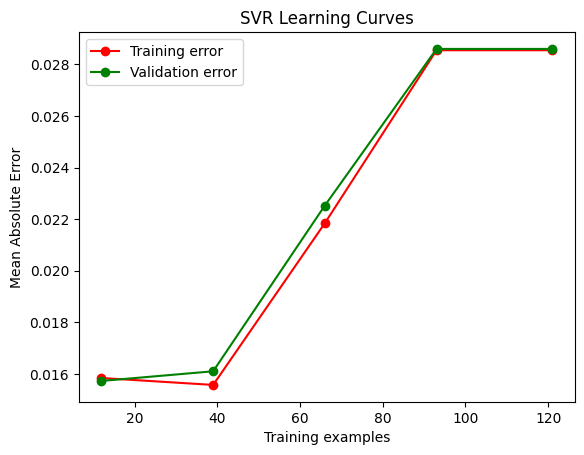
\includegraphics[scale=0.3]{images/SVR_lc.png} & 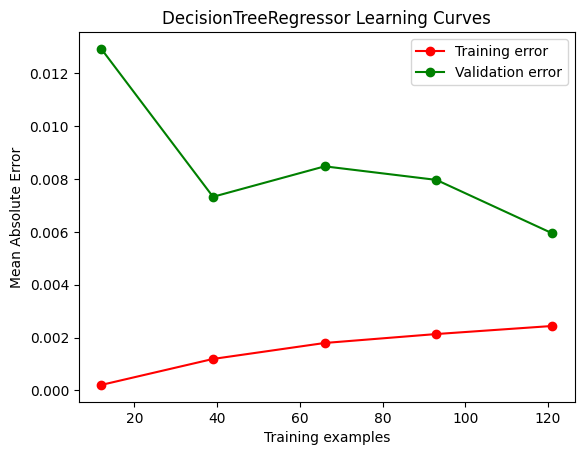
\includegraphics[scale=0.3]{images/DecisionTree_lc.png} \\
        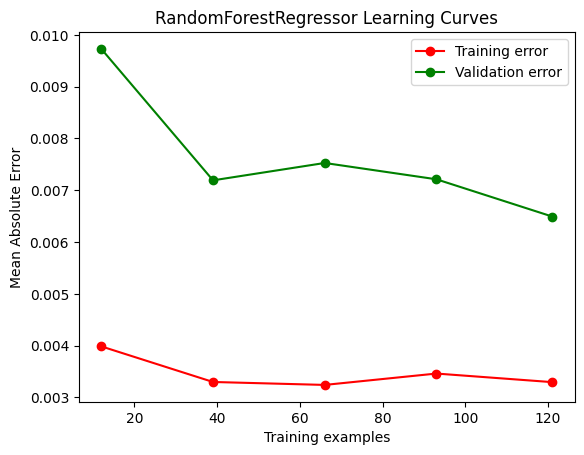
\includegraphics[scale=0.3]{images/RandomForestRegressor_lc.png} & 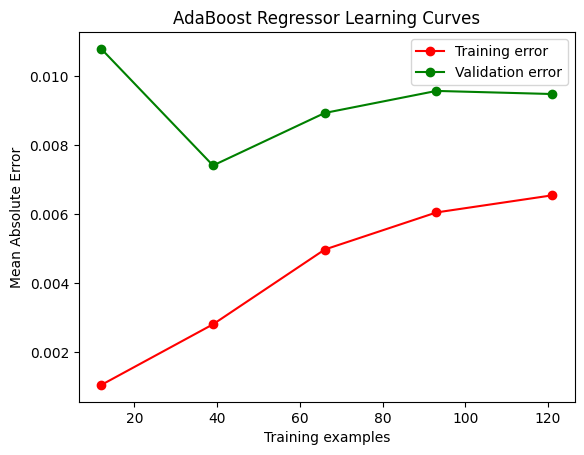
\includegraphics[scale=0.3]{images/AdaBoostRegressor_lc.png} \\
    \end{tabular}
    \caption{Learning curve dei regressori}
    \label{tab:lc}
\end{table}

\subsection{Analisi dei risultati}


    \paragraph{\textbf{SVR}.}
    Dal punto di vista delle metriche il regressore SVR ha ottenuto i peggiori risultati in termini di MAE, RMSE e MSLE. La learning curve mostra che il modello è in overfitting, infatti gli errori aumentano all'aumentare del numero di istanze.
   
   
    \paragraph{\textbf{Decision Tree Regressor}.}
    Dal punto di vista delle metriche, il Decision Tree Regressor ha ottenuto i migliori risultati. 
    La learning curve mostra una curva di training che aumenta all'aumentare del numero di istanze, mentre la curva di validation diminuisce. Le due curve si avvicinano, ma non si sovrappongono. Sembra esserci un leggero underfitting.
    \paragraph{\textbf{Random Forest Regressor}.}
    Dal punto di vista delle metriche il Random Forest Regressor risulta essere il secondo miglior modello.
    La learning curves di train e di validation set diminuiscono entrambe all'aumentare del numero di istanze, ma non si sovrappongono. Anche qui sembra esserci underfitting.
    \paragraph{\textbf{AdaBoost Regressor}.}
    Dal punto di vista delle metriche il AdaBoost Regressor ha ottenuto risultati peggiori rispetto al Random Forest Regressor ma migliori rispetto al SVR.
    La learning curve mostrano che il modello non è riuscito a generalizzare bene


\subsection{Conclusioni}
Il dataset sembra essere troppo piccolo per poter generalizzare bene i modelli. Inoltre, il dataset è molto sbilanciato, con pochi valori per ogni feature. Questo potrebbe essere un motivo per cui i modelli non generalizzano bene. Inoltre, i modelli non sono stati ottimizzati, quindi potrebbero essere migliorati mediante ricerca di iperparametri.
Per i risultati attuali, il Decision Tree Regressor è il modello migliore.